\documentclass[12pt]{Report}
\usepackage{graphicx}
\begin{document}
\title{Assignment 1 : CS 751 }
\maketitle


\section{Part 1}

\paragraph{Extracting and Storing  Tweets}
I have created a twitter developers account and created consumer key , consumer secret key , authorization token and authorization secret key . Secret keys for API are collected after registering the application in twitter. I have written a program called "extractLinksFromTwitter.py" is in "pythoncodes" folder . This code extracts the 10000 tweets with links from twitter . These links are extracted using the above keys which i have mentioned . This code imports tweepy library to get the links . All the tweets with links and tweet id's  are extracted to "tenthousandtweetLink" which is present in "input-output files" folder.  The above script executed for 30 minutes in order to extract the 10000 tweets. 

\paragraph{Curl to record HTTP Headers}

In order to chase down all the redirects , i have written a code called "urlResponseAfterCurl.py" which is located in the folder "pythoncodes" .
This code loops through all the links one by one and records the HTTP STATUS information into an array for each link. This is finally extracted to a file named "responseAfterCurlCalls.txt" which is located in the folder "input-output files".

\paragraph{Unique and Duplicate Url count } 

I have written a code named "uniqueUrlCount.py" which is located in "pythoncodes" folder . This code takes the input file named " responseAfterUrlCalls.txt" and iterates through each link and adds it to "set()"  type variable. The "set()" type is more like an array but it only allows the user to insert unique elements into it . By this we will be able to get the unique url's and duplicate url's count.

\paragraph{Histogram of count of Redirects }

I have written a code named "ExtractStatusCodeAndRedirectCount.py" which is located in "pythoncodes" folder . This code takes "responseAfterCurlCalls.txt" as input and calculates the number of redirects for each link and copies to a file named "redirectCountList.txt" . It also copies all the status codes for each link into statusCodeList.txt file . These output files are located in "input-output file" folder.
I have written two scripts named "histogramScriptForRedirectCount.R" and "histogramscriptForStatusCodes.R" in RStudio which is located in histogram folder  which takes the above  input files and outputs the histogram in png format images named "StatusCodeHistogram.png" and "urlRedirectCount.png" which is located in histogram folder.
The below are the histograms for status codes and number of redirects.



\newpage
\subsubsection{Histograms}
\begin{figure}[ht]    
    \begin{center}
        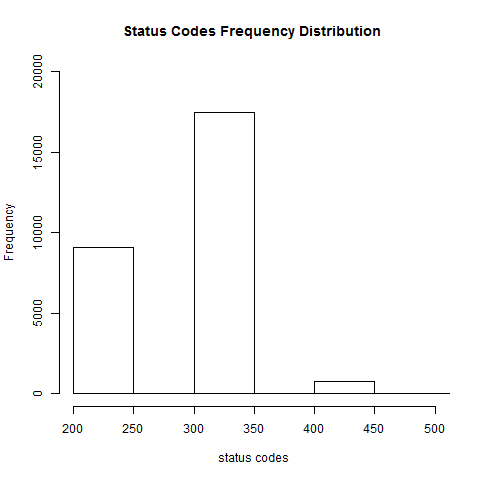
\includegraphics[scale=0.60]{StatusCodeHistogram.png}
        \caption{Histogram 1}
        \label{StatusCodes Frequency Distribution}
    \end{center}
\end{figure}
\newpage
\begin{figure}[ht]    
    \begin{center}
        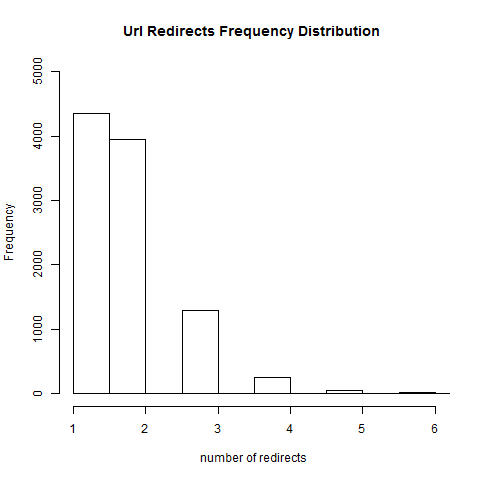
\includegraphics[scale=0.60]{urlRedirectCount.png}
        \caption{Histogram 2}
        \label{Count of number of redirects}
    \end{center}
\end{figure}
\newpage


\section{Part2}

\paragraph{Carbondate to estimate age of link}

First i have downloaded the carbondate master from github . 
Added my bitly access token which i have generated using twitter account to the configuration file. Then i have edited the "local.py" (which is  located in the folder "pythoncodes") in such a way that it reads in all the 10000 links from a file named "responseAfterCurlCalls.txt " which is located in folder "input-output files" and outputs the estimated carbon date for each link into "carbondatedata.txt" file . In order to decrease the execution time i have created 10 such local.py files , executed them simultaneously and  extracted the carbondate to 10 output files and finally merged them into one file named "carbondate.txt".

\subsection{Age tweet - Age Link}

I have written a code named "AgeExtraction.py" which calculates the age of tweet and age of link. Also, the delta(age tweet - age link) is calculated for each link and pushed to a file named "AgeExtract.txt".\\
I have written a small snippet in Rstudio in order to get a histogram for delta of age . This script reads the "AgeExtract.txt " file as input and outputs the histogram in a png format .

The histogram for delta (age) is  shown below.

\newpage
\begin{figure}[ht]    
    \begin{center}
        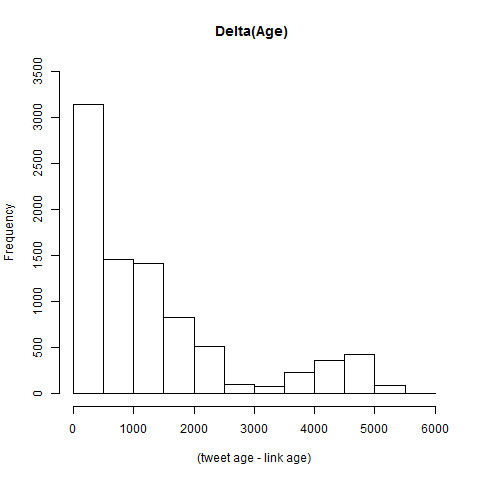
\includegraphics[scale=0.60]{delta--age.png}
        \caption{Histogram 2}
        \label{Count of number of redirects}
    \end{center}
\end{figure}
\newpage



\subsection{Statistics for the delta(age) }

I have calculated the mean , median , stddev , stderr for the delta values produced in AgeExtract.txt file. I have calculated these values with the help of excel formulas . All these data is located in "StatisticsDataForDeltas.xlsx" which is located in "input-output files" folder .\\

mean :	1330.417445\\
median: 	882\\
stddev: 	1377.175273\\
stderr:	14.79295098\\






  



\end{document}


